% This file is not used
\subsection{Energy Improvement from MCRP}

Multichannel protocol not only could reduce the end to end delay, it also helps to improve the nodes energy efficiency by ensuring minimal packet retransmissions thus energy consumption.
MCRP implements Contiki's existing energy module, Powertrace.
Powertrace uses the software based on-line energy estimation mechanism \cite{dunkels2007software} to estimate the node's current energy consumption in real time. 
The energy estimation module uses time measurements that can be directly obtained from the microprocessor on-chip timer when the component is switched on to produce a time stamp. The time difference from when the component was on and when it later is switched off is computed. The current draw of the component listed in the TelosB data sheet is used to compute the total energy consumption estimation, $E$. 

\begin{equation}
E = (I_{m}t_{m} + I_{l}t_{l} + I_{tx}t_{tx} + I_{r}t_{r} +  \sum_{i}I_{c_{i}}t_{c_{i}}) \times{V}
\label{energyModel}
\end{equation}

Equation \ref{energyModel} shows the energy consumption model given in \cite{dunkels2007software}  
where $V$ is the supply voltage, $I$ is the current draw and $t$ is the active time computed in Powertrace for $m$ the microprocessor, $l$ the microprocessor in low power mode, $tx$ the communication device in transmit mode, $r$ the communication device in receive mode and $c_{i}$ for other components such as sensors and LEDs. The values of $I_{m}$, $I_{l}$, $I_{tx}$ and $I_{r}$ are device dependent. 

Powertrace is used to compute the energy consumption estimation of the network. However, the nodes do not have enough capability to compute their individual energy consumption. In order to estimate the energy taken from the sender to the receiver, each node sends their energy values to LPBR regularly as MCRP has a centralised controller. This enables LPBR to predict the energy drain if the routes have high interference or packet losses. LPBR is able to compute the end to end energy consumption on each routes and estimate the nodes battery level based on the energy values. Each node sends the energy value of its packet transmission, packet forwarding and total time value that the radio has been on from the beginning to LPBR for energy consumption computation.
By doing that, the nodes knowledge of its energy level is kept at minimum. 

In order to calculate accurate energy consumption for specific packet transmission, the unicast packet type is separated into normal unicast and control messages unicast. The unicast packet from the application layer (normal unicast) is set as \textit{unicastMsg = 1}, which the value is 0 by default to represents other unicast packets. This allows the energy of the transmission packet to be calculated separately without including other control messages that could be sent right after or before the normal packet transmission. This is done to avoid inaccurate energy spent as control messages are only being sent periodically unlike the normal packet that are sent frequently. It also enables retransmit packets to be included as the current transmission packet energy. This will alert the LPBR on the current condition of the node with much higher energy consumption than the usual energy per packet because of the retransmissions. The $unicastMsg$ value is reset when the link layer acknowledgement is received or the maximum number of retransmission is reached. 

\subsection{Energy Performance Evaluation}
 
The energy consumption in MCRP in term of transmission per packet, forwarding packets energy and total energy used are computed to prove that multichannel helps to prolong the network lifetime by using the energy more efficiently than in a single channel network. Each node sends one packet per minute, 350 packets in total throughout the simulation period. Equation \ref{energyModel} is used to calculate the nodes energy consumption. The energy consumption of each node is computed by the LPBR based on the information contained in the transmitted packet. The maximum number of hops in the simulation is 3 hops. The results of a single channel with no interference is used as the base case as it is the ideal energy consumption value. The results are also compared to the energy of a single channel with moderate and extreme interference, and MCRP for multi channels.

\subsubsection{Energy Per Packet Performance}

\begin{figure}
\centering
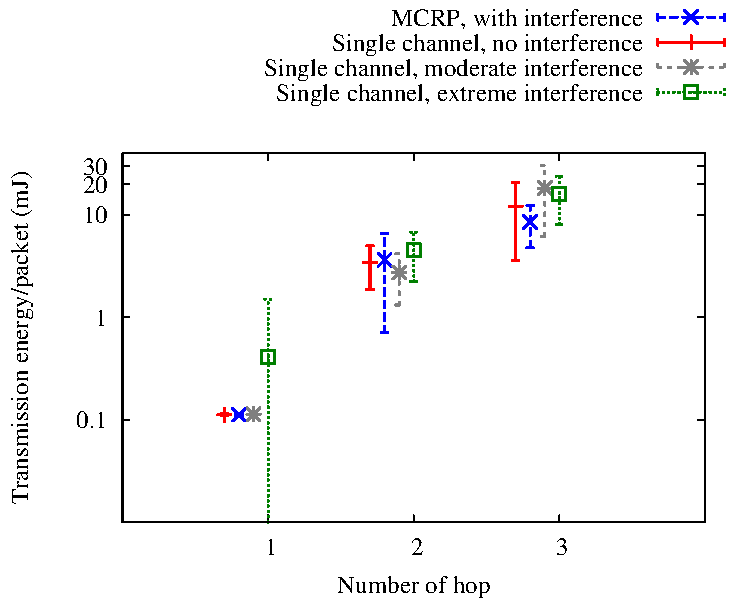
\includegraphics[width=0.45\textwidth]{figures/perPktEnergy.pdf}
\caption{Simulation: The energy consumption per packet in different number of hops}
\label{fig:energyPerPkt}
\end{figure}

Figure \ref{fig:energyPerPkt} shows the transmission energy per packet for nodes that are 1, 2 and 3 hops away from the LPBRs. From the figure, it can be concluded that less transmission energy is used when there is less number of hops. However, in a large scale network, the number of hops cannot be reduced as not all nodes would be in the range or directly connected to the destination node. Thus, the node's next hop should be selected carefully to avoid nodes that have higher interference rate.

In the 1 hop case, it can be seen that the nodes consumed approximately similar energy in all cases. As the nodes are one hop to the destination (LPBR), it was not affected by the interference except for a slight variation in the single channel with extreme interference case. 
Nodes that are 2 and 3 hops away show higher values of per packet energy transmission.
This is because of the interference near to the nodes. The nodes are unable to detect the exact wake-up time for the nodes thus, the nodes have to transmit in a longer period to ensure the packet gets transmitted. In the one hop graph, the energy can be kept at minimum because the LPBR is always awake to accept packet as it is fully powered unlike the other nodes that have to switch the radio off when there are no transmissions and receptions taking place to save the energy.

In the 1 and 2 hops, MCRP shows approximately similar transmission energy consumption to the base case. 
In 3 hops, the energy per packet in the single channel with moderate and extreme interference are much higher than the energy used by the base case and MCRP. This shows that the energy per packet depends on the number of hops and the interference that affect the routes. Multichannel helps to mitigate the effect of interference, thus reducing the transmission energy taken to send a packet especially when there are several hops involved.

\subsubsection{Total Energy Consumption}

\begin{figure}
\centering
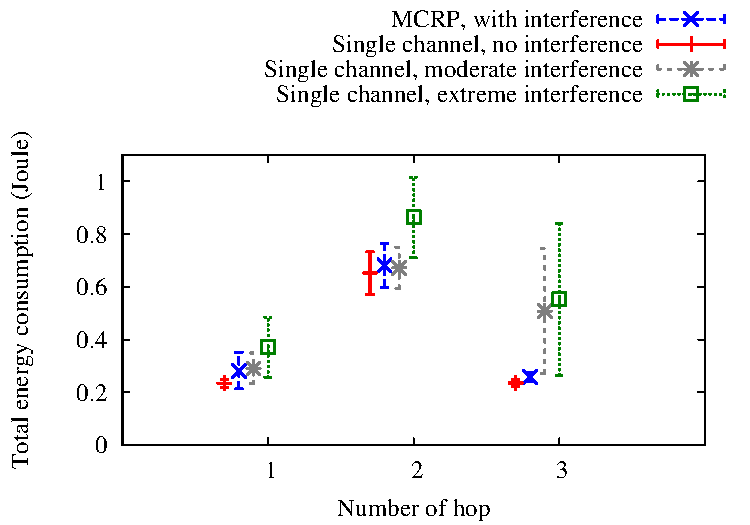
\includegraphics[width=0.45\textwidth]{figures/totalEnergy.pdf}
\caption{Simulation: The nodes total energy consumption}
\label{fig:allNodesEnergy}
\end{figure}

Figure \ref{fig:allNodesEnergy} shows the total energy consumption in the simulation including retransmissions and control packets energy.  
In 1 hop, it can be seen that in all cases, the total energy taken are approximately similar with a small standard deviation. The single channel with extreme interference case however, requires higher energy consumption than in other cases.
In 2 hops, it shows high increase in energy usage. The reason for this is because the 2 hops nodes are used as forwarding nodes. The 3 hops nodes do not act as forwarding nodes thus the reason for the lower total energy consumption.
The energy consumption is improved when using MCRP than a single channel with interference. This improvement can be clearly seen in the 3 hops nodes where MCRP uses 3 times less energy than in the single channel cases of an approximate 0.6 Joules as these nodes use more energy during interference for retransmissions. If the retransmissions fail, the packet is dropped and the energy used during the retransmissions is wasted. The total energy consumption graph shows all energy spent when the nodes are awake, including forwarding and failed packets transmission.

\subsubsection{Forwarding Energy Analysis}

\begin{figure}
\centering
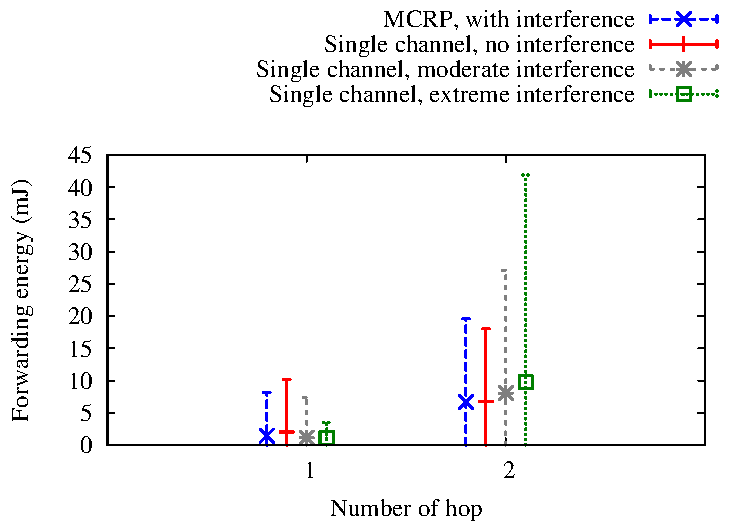
\includegraphics[width=0.45\textwidth]{figures/fwdEnergy.pdf}
\caption{Simulation: The nodes forwarding energy}
\label{fig:allNodesFwdEnergy}
\end{figure}

Figure \ref{fig:allNodesFwdEnergy} shows the energy used in forwarding packets for the 1 and 2 hops nodes. The 3 hops nodes in the simulation do not forward packets. The 1 hop nodes use less energy than the 2 hops nodes as the nodes only need to check if the channel is being use by the other node before it can forward to the LPBR. LPBR waits for incoming packet thus the nodes could send the packet with less waiting time as LPBR radio is always on. 
In order to be able to forward the packets, the nodes have to be awake for longer time and ensure the intermediate node is also awake and ready to accept the packets. Thus forwarding could require more energy consumption than an end to end packet transmission. By increasing the number of nodes thus children, the nodes will use more energy in order to forward the packets. The forwarding energy consumption contributes to the most energy used by the nodes.  
Even though MCRP does not show a lot of improvement, it shows lower deviation compared to the single channel with extreme interference.
In the base case, the energy consumption varies as the nodes are interfering with each other even without external interference during transmissions.

The simulation results showed that MCRP consumes less energy than in other cases when there is interference as the effect of multichannel. MCRP has similar energy consumption values as in the base case, a single channel without interference. This shows that multichannel helps to reduce the energy wasted due to interference. In order to increase the energy efficiency thus network lifetime, MCRP needs to reconstruct the topology based on the energy consumption, residual energy of the nodes and the link conditions gradually to avoid breaking any current connectivity.
